\chapter{Simulation}

%--------------------------------------------------------------------------------------------------------
% 		Intro
%--------------------------------------------------------------------------------------------------------

This chapter provides an overview of the two simulations which were created.
These simulations are intended to be as realistic as possible and involve random movement of ferry nodes.
The ferries were assumed to be vehicles which defined their speed.
A number of scenarios were tested for each simulation, the parameters varied are explained in section \ref{sec:metrics}.

%--------------------------------------------------------------------------------------------------------
% 		Topology
%--------------------------------------------------------------------------------------------------------
\section{Network Model}
\label{sec:main_net_model}

This section outlines the two network models defining each simulation. 
Their difference lies on the number of ferry and gateway nodes.
The parameters common between each are explained in section \ref{sec:commonsettings}.

\subsection{Scenario 1}		%1 gateway, 1 ferry

The first simulation was created with one gateway node, one ferry node, and ten source nodes.
The network model may be seen in figure \ref{fig:scenario2}.
The gateway is placed in the center of the map and the ferry node starts next to it.
Source nodes are more or less evenly distributed and are placed such that they are out of direct communication range.

\begin{figure}[ht]
    \centering
    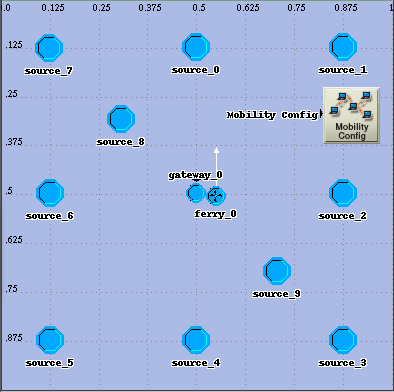
\includegraphics[width=0.6\textwidth]{images/scenario2-top.png}
    \caption{Simulation 1 - Network Model (1 Gateway, 1 Ferry)}
    \label{fig:scenario2}
\end{figure}

\subsection{Scenario 2}		%2 gateways, 2 ferries

The second simulation was created with two gateway nodes, two ferry node, and ten source nodes.
The network model may be seen in figure \ref{fig:scenario3}.
The gateways are placed in opposing quadrants, while both ferries start from the center.
Source nodes and gateways are more or less evenly distributed and are placed such that they are out of direct communication range.

\begin{figure}[ht]
    \centering
    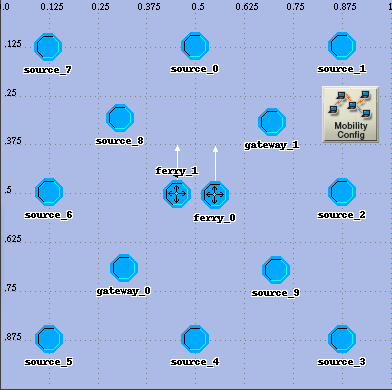
\includegraphics[width=0.6\textwidth]{images/scenario3-top.png}
    \caption{Simulation 2 - Network Model (2 Gateways, 2 Ferries)}
    \label{fig:scenario3}
\end{figure}

\subsection{Common Settings}
\label{sec:commonsettings}

Some of the settings and characteristics common to all the topologies are the following:
\begin{itemize}
	\item All ferries move in random directions and have a varying speeds of 36kph - 72kph in uniform distribution.
	\item The size of both maps is 1km x 1km
	\item Properties are updated every 2 seconds with a variance of 0.1 seconds
	\item Simulations are run for 90 minutes. 
	Property updates were disabled for the last thirty minutes in an effort to obtain statistics valid for a simulation of indefinite length. 
\end{itemize}

%--------------------------------------------------------------------------------------------------------
% 		Metrics and Results of Interest 
%--------------------------------------------------------------------------------------------------------
\section{Metrics and Results of Interest }
\label{sec:metrics}

Two metrics are of primary interest when analyzing the network, update success rate and delay.

\subsection{Update Success Rate}
\label{sec:packetloss}

Update success rate, or alternatively update loss, is of central importance in the network.
It is primarily affected by memory limits imposed by the ferry but is also affected by the number of ferry and gateway nodes.
Defining success rate is somewhat complicated as updates may be intentionally discarded before they reach a gateway if they are out of date.
Additionally, updates may be duplicated multiple time as ferries exchange messages.
Finally, discarding updates with a key update number less than the most recent key update number received by the gateway is desired behaviour.
As such, the following conditions are used to determine success rate which is measured as \emph{success}, \emph{failure} or \emph{no value} for each key update generated by every source node property.

\begin{itemize}
\item For updates which reach the gateway:
	\begin{itemize}
	\item If the update has a key update number greater than the last update received by the gateway (for a given source id and property key) the update counts as a \emph{success}.
	\item If the update has a key update number equal to or less than the last update received by the gateway (for a given source id and property key) the update is not considered and counts as \emph{no value}.
	\end{itemize}
\item For updates which do not reach the gateway and are discard by every ferry node:
	\begin{itemize}
	\item If the update has a key update number greater than the last update received by the gateway (for a given source id and property key) the update counts as a \emph{failure}.
	\item If the update has a key update number equal to or less than the last update received by the gateway (for a given source id and property key) the update is not considered and counts as \emph{no value}.
	\end{itemize}
\end{itemize}

\subsection{Delay}
\label{sec:delay}

The number of ferries and gateways is the primary parameter affecting delay, however, ferry memory limits also play a role.
Delay is defined as the time an update takes to reach the gateway after it has been generated by a source node.
Only updates which are successfully delivered (as defined in section \ref{sec:packetloss}) 
count towards delay.
As such, it is important for results of delay to be considered within the context of update success rate.
It should be noted that the lower bound on delay is the time it physically takes the ferry to move between the source node and gateway.

\subsection{Simulation Parameters Varied}

The following parameters were varied to create additional scenarios for each simulation as presented in section \ref{sec:main_net_model}. 
Their impact on success rate and delay (from sections \ref{sec:delay} and \ref{sec:packetloss}) were considered.
  
\subsubsection{Memory Limit}
\label{sec:mainMemLimit}
The memory limit, also referred to as capacity, is the buffer size of the ferry.
It limits the number of unique updates which can be stored at once.
It is set in number of updates, not bytes, and hence is somewhat unrealistic.
It is sufficient for the purposes of this scenario however.

\subsubsection{Seed - Effect of Randomness}
Since ferry movement is random and the number of gateways is limited, it is important to consider multiple random when simulating in OPNET. 

\subsubsection{Source Node Storage}
\label{sec:source_node_storage}
The node models and algorithm presented thus far has assumed that only ferries store updates. 
A modified node model which allows source nodes to store updates was also considered.
The effect of enabling source node storage was examined.

